\subsection{Генетический алгоритм}
\label{sec:1c}

Использование генетического алгоритма для оптимизации кластерных структур
началось в 90-х годах с работ Хартке (для кремниевых кластеров малого размера)
\cite{Hartke1993} и Вильямса (для молекулярных кластеров) \cite{Xiao1993}. В обоих
случаях структура кластеров была закодирована с помощью бинарных строк. При этом
генетические операторы использовали бинарные операции над ними. Важным улучшением
генетического алгоритма для кластерной оптимизации стало использование действительных
Декартовых координат для представления кластеров. Этот подход был предложен
Зейри \cite{Zeiri1995} и позволил снять ограничение на бинарное кодирование генов.

Следующий шаг в развитии генетических алгоритмов для кластерной оптимизации был
предложен Дивеном и Хо \cite{Deaven1995}. Главной идеей является нахождение локального
минимума общей потенциальной энергии кластера для каждого кластера, полученного
с помощью генетического алгоритма на очередном шаге. Это позволяет значительно
уменьшить пространство возможных решений для генетического алгоритма.

Дивен и Хо также предложили трехмерный оператор скрещивания, которую назвали
"разрез и склеивание" ("cut and splice"). Этот оператор, который использовался
в большинстве последующих работ по кластерной оптимизации, привносит больше 
физического значения в процесс скрещивания. Этот механизм будет описан более
подробно позже.

На основе вышеперечисленных разработок в области генетических алгоритмов для
кластерной оптимизации Джонстон и др. предложили генетический алгоритм,
который назвали "бирмингемским" \cite{Johnston2002}. Именно этот алгоритм и был
выбран в качестве основы для реализации экспериментального программного обеспечения.
%TODO: не надо кодировать/раскодировать хромосомы

Необходимо заметить, что генетический алгоритм является стохастическим алгоритмом
и результаты его выполнения могут отличаться от запуска к запуску, в отличие от
использованного метода молекулярной динамики, где результат полностью определяется
входными данными. Также необходимо понимать, что равновесная конфигурация, полученная
в результате работы генетического алгоритма может значительно отличаться от начальной
конфигурации, заданной пользователем опять же в силу стохастической природы генетического
алгоритма.

Общая схема работы приложения, реализующего генетический алгоритм, показана на
рис. \ref{block_gen}.

\begin{figure}[ht!]
 \begin{center}
 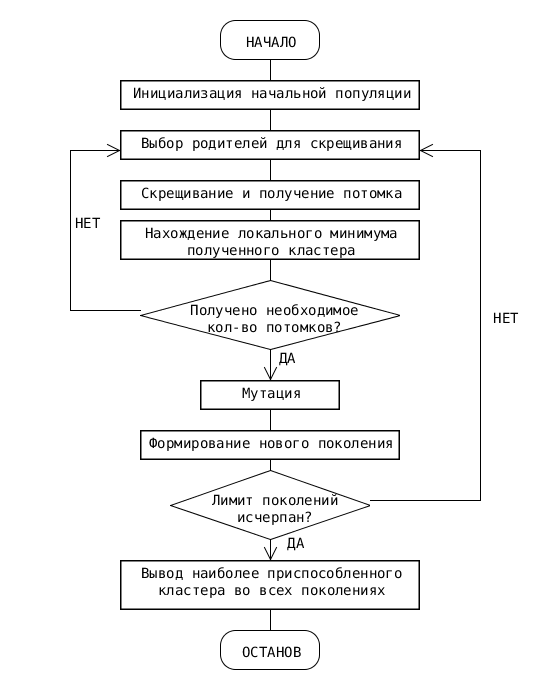
\includegraphics[height=0.65\textheight]{FIGs/gen_alg_block.png}
 \end{center}
 \caption {Блок-схема реализации генетического алгоритма}
 \label{block_gen} 
\end{figure}

Ниже следует более подробное описание каждого из этапов, указанных на блок-схеме.

\subsubsection {Инициализация}.
В бирмингемском алгоритме для кластера заданного размера (состоящего из $N$ элементов)
генерируется $N_{clus}$ (от 10 до 30) кластеров случайным образом для формирования начальной
популяции. В реализованном приложении пользователь имеет возможность задать начальное
приближение для координат кластеров, поэтому нет необходимости генерировать все
кластеры начальной популяции случайным образом. С другой стороны, нежелательно, чтобы
начальная популяция состояла из полностью идентичных особей -- в таком случае разнообразие
внутри популяции будет недостаточным. Вместе с тем разнообразие важно для генетических алгоритмов
потому, что перекрёст генов в гомогенной популяции не несёт принципиально новых решений. В приложении
реализован комбинированный подход: часть кластеров в начальной популяции задается
случайным образом, а остальная часть состоит из кластеров с начальным приближением,
заданным пользователем. Процентное соотношение между частями задаётся пользователем.

На генерируемые случайным образом кластеры накладываются два типа ограничений:
минимальное межатомное расстояние, а также максимальные значения координат атомов
по каждому из измерений. Такие ограничения позволяют генерируемым классам быть соразмерными
с начальным приближением, заданным пользователем, и вследствие быть более подходящими
кандидатами для скрещивания.

Все кластеры начальной популяции минимизируются к точке локального минимума с помощью алгоритма,
описанного в %TODO: ref.

\subsubsection {Функция приспособленности}

Функция приспособленности конкретной особи это оценка качества особи с точки зрения
конкретной задачи. В данном случае, кластеры с наименьшей энергией (наименьшей $V_{clus}$)
имеют наибольшее значение функции приспособленности. Генетический алгоритм использует
динамическое масштабирование приспособленности, основанное на нормализованном значении
энергии, $\rho$:

\begin{equation}
  \rho_{i} = \frac{V_{i} - V_{min}}{V_{max}-V_{min}}
\end{equation}

где $V_{min}$ и $V_{max}$ минимальное и максимальное значение энергии кластеров в
текущей популяции соответственно.

\subsubsection {Скрещивание}

В приложении реализованы два метода скрещивания: биномиальный и ``разрез и склеивание''.
Используемый метод задается пользователем и используется на всем протяжении работы
генетического алгоритма.

Биномиальный метод описан в работе \cite{Zaharie2007} и является универсальным методом,
применимым при реализации любого генетического алгоритма. Этот метод может быть описан
следующей последовательностью шагов:

\begin{enumerate}
  \item{Выбрать случайное число $k$ в интервале $[0, N_{atom} - 1]$.}
  \item{Сгенерировать последовательность $\lbrace r_{i}, i=1 \cdots N_{atom} \rbrace$
    случайных вещественных чисел в диапазоне $(0,1)$.}
  \item{$\forall i, i \neq k$: положить $i$-ый атом потомка равным $i$-ому атому первого
      родителя, если $r_{i} < binom\_rate$ или равным $i$-ому атому второго родителя
    в противном случае.}
  \item{Положить $k$-ый атом потомка равным $k$-ому атому второго родителя.}
\end{enumerate}

Значение параметра $binom\_rate$ задается пользователем.

Метод ``разрез и склеивание'' представляет собой вариант оператора скрещивания,
предложенного Дивеном и Хо \cite{Deaven1995}. К кластерным структурам обоих родителей сначала
применяются случайные повороты вокруг двух перпендикулярных осей, а затем оба кластера разрезаются
горизонтально параллельно плоскости $xy$ посередине и соответствующие части склеиваются вместе,
как показано на рис. \ref{cut_and_splice}. Таким образом, метод пытается учитывать специфику
обрабатываемых данных и не является универсальным методом скрещивания.

Важным моментом в процедуре скрещивания является выбор родителей. Разработано много методов для селекции
родителей, обзор и сравнение которых приведен в \cite{Blickle1995}. В настоящем приложении
были реализованы два метода: турнирный и метод колеса рулетки. Используемый метод селекции
задаётся пользователем.

В турнирном методе несколько кластеров выбираются случайным образом, чтобы
образовать турнирную группу. Два кластера с минимальной энергией затем
выбираются из этой группы в качестве родителей. При такой схеме кластеры с
наибольшим значением функции приспособленности имеют высокую вероятность быть
выбранными для скрещивания и таким образом передать особенности своей структуры
следующим поколениям.

Алгоритм селекции методом колеса рулетки описан в примере минимизации функции с помощью
генетического алгоритма в параграфе \ref{sec:1d}.

В результате процедуры скрещивания появляется один новый потомок. Выбранный метод применяется
столько раз, сколько потомков необходимо получить в следующем поколении.
Для каждого кластера-потомка затем применяется градиентный метод, описанный в, %TODO: reference
чтобы структура кластера соответствовала ближайшему локальному минимуму потенциальной энергии.

\begin{figure}[h!]
\centering
  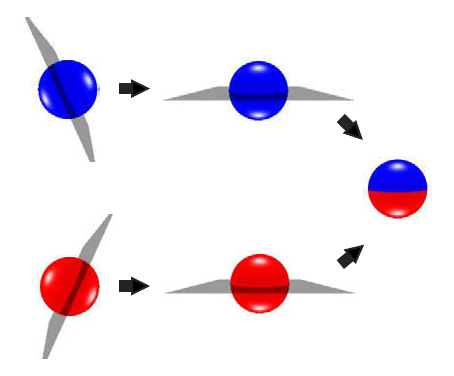
\includegraphics[width=0.5\textwidth]{./FIGs/cut_and_splice.png}
\caption{Оператор скрещивания "разрез и склеивание"}
\label{cut_and_splice}
\end{figure}

\subsubsection {Мутация}

Несмотря на то, что операция скрещивания приводит к перемешиванию генетического материала
в кластерах-потомках, нового генетического материала при этом не появляется. Для того, чтобы
поддержать разнообразие особей в популяции, вводится новый оператор мутации. Каждая особь
имеет некоторую вероятность подвергнуться мутации ($P_{mut}$), которая возмущает некоторые или
все позиции атомов внутри кластера. После мутации, каждая особь локально минимизируется.

В приложении использовано несколько видов мутации:

\begin{itemize}
  \item{Перемещение атомов.Данная мутация заменяет координаты некоторых атомов кластера
случайными значениями. Количество атомов для замены координат было выбрано равным
трети ($N/3$) от общего количества атомов.}
\item{Вращение.Происходит поворот верхней части кластера вокруг оси $z$ на случайный угол
  относительно нижней части кластера.}
\item{Замена кластера.Происходит замена целого кластера на новый, координаты которого заданы
  случайным образом.} 
\end{itemize}

Перечисленные мутации приводят к достаточно значительным изменениям генетического материала.


\subsubsection {Последующие популяции}

Новая популяция представляет собой объединение некоторого количества ($N_{clus}$) кластеров
с большими значениями функции приспособленности, некоторого количества потомков ($N_{off}$),
а также некоторого количества мутировавших кластеров.

Процесс последовательного скрещивания, мутации и селекции происходит заданное количество
раз ($N_{gen}$).
